% Figure M4, generated by experiments/m4_facet_vs_sae.py.
\begin{figure}[t]
  \centering
  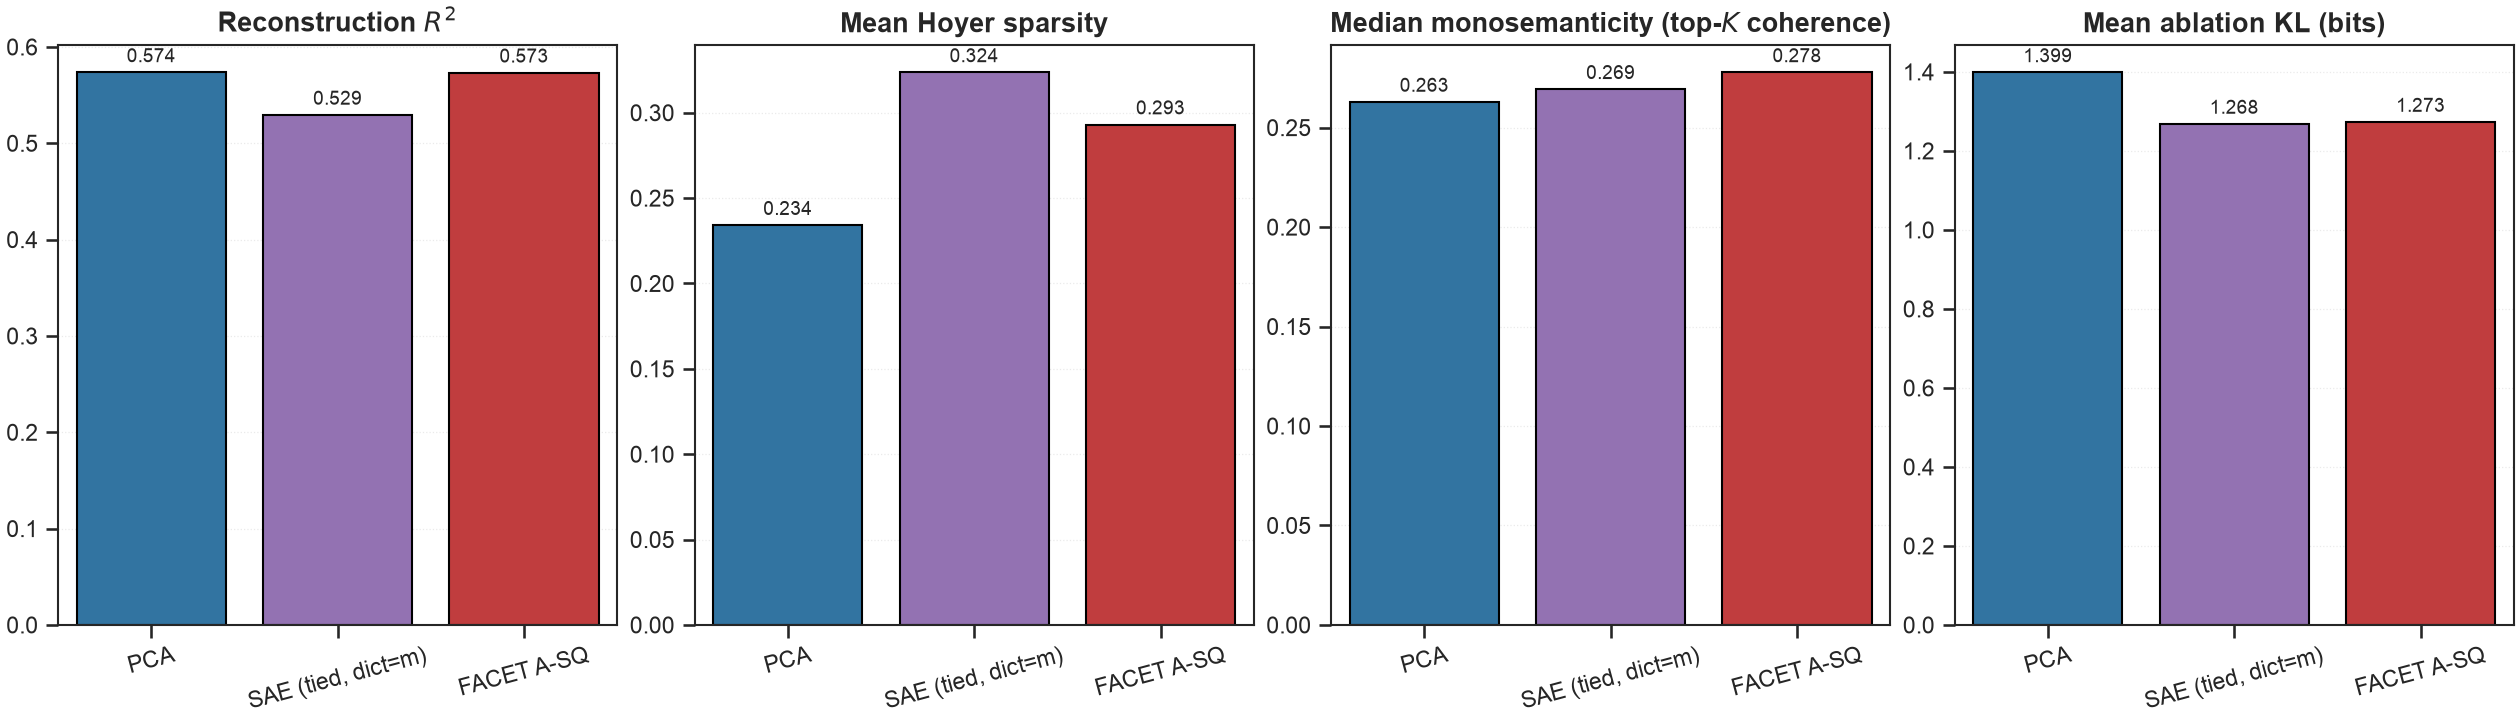
\includegraphics[width=\linewidth]{../shared/figures/generated/m4_facet_vs_sae.png}
  \caption{\textbf{M4, FACET vs tied sparse autoencoder at matched $m{=}32$} on GPT-2 small block 4 \texttt{attn\_out}. A tied-decoder SAE (dictionary size $={}m$, $L_1$ coefficient $0.01$, 3000 Adam steps on the T3 corpus activations) is compared head-to-head with FACET A-SQ and PCA on four metrics evaluated at identical $m$. Reconstruction $R^2$: PCA $0.574$, FACET $0.573$ (tied), SAE $0.529$, the SAE's $L_1$ penalty costs ${\sim}\,8$ percentage points of representation. Mean Hoyer sparsity per component: SAE $0.324$, FACET $0.293$, PCA $0.234$. Median monosemanticity (M2 coherence): FACET $0.278$, SAE $0.269$, PCA $0.263$. Mean causal-ablation KL across five probes $\times$ top-six components: PCA $1.40$ bits, FACET $1.27$, SAE $1.27$. Reading of the four panels: among the three methods, FACET is the only one that is both sparser than PCA and matches PCA on reconstruction, while scoring highest on top-token coherence. The SAE pays a reconstruction cost for its $L_1$-driven sparsity.}
  \label{fig:m4-facet-vs-sae}
\end{figure}
